\documentclass[10pt]{article}
\usepackage[utf8]{inputenc}
\usepackage[margin=1in]{geometry}
\usepackage{hyperref}
\usepackage{fixme}
\usepackage{csquotes}
\usepackage{todonotes}
\usepackage{listings}
\usepackage{biblatex}
\usepackage{csvsimple}
\usepackage{graphicx}
\usepackage[english]{babel}
\fxsetup{
    status=draft,
    author=,
    layout=inline,
    theme=color
}
\definecolor{fxnote}{rgb}{0.8,0,0}
\title{Introduction to the Julia Language}
\author{Colin Beardshear\\ \texttt{crbeardshear@ucdavis.edu} \and
Alen Yu\\ \texttt{lenyu@ucdavis.edu} \and
Devon Johnson\\ \texttt{dnrjohnson@ucdavis.edu}
}
%custom definition so Julia code is displayed more cleanly
\lstdefinelanguage{Julia}%
  {morekeywords={abstract,break,case,catch,const,continue,do,else,elseif,%
      end,export,false,for,function,immutable,import,importall,if,in,%
      macro,module,otherwise,quote,return,switch,true,try,type,typealias,%
      using,while},%
   sensitive=true,%
   alsoother={$},%
   morecomment=[l]\#,%
   morecomment=[n]{\#=}{=\#},%
   morestring=[s]{"}{"},%
   morestring=[m]{'}{'},%
}[keywords,comments,strings]%

\lstset{%
    language         = Julia,
    basicstyle       = \ttfamily,
    keywordstyle     = \bfseries\color{blue},
    stringstyle      = \color{magenta},
    commentstyle     = \color{green},
    showstringspaces = false,
}

%citations:
\addbibresource{juliadevs.bib}

\begin{document}
\maketitle

\fxnote{I have just ported over the google doc. This isn't by any means the final formatting. (You can use this command to write in red text for suggested changes, etc.)}
\todo{You can also use todo's like this.}
%comments are written like this

\section*{\normalsize History and motivation for Julia -- why have yet another scripting language?}

Julia is meant to be the best of both worlds between:
\begin{itemize}
\item The productivity of dynamic, higher level languages such as Python, R, and MATLAB.
\item The performance of lower level languages such as C and Fortran.
\end{itemize}
Julia was designed by Jeff Bezanson, Stefan Karpinski, Viral Shah, Alan Edelman. The designers wanted a language where the they could have the speed of C and the dynamic types and expressiveness of Ruby. They wanted to keep a familiar syntax of MATLAB since many were MATLAB power users. They also wanted a general purpose language like Python but also a powerful but easy to pick up statistical tool like R.

Previously, many developers would use both higher and lower level languages for their merits above; by creating a dynamic, higher level language which is better suited to computationally intensive examples, developers are able to avoid a `Two-Tiered Architecture'\cite{juliadevs}. This boosts both productivity (more than would already be gained by using a higher level language) and readability.

\section*{\normalsize General structure: What does it look like syntactically? Does it have any unusual language constructs?}

	The general syntax of Julia looks like MATLAB but Julia has several language constructs and conventions that make it unique. <Julia is dynamically typed>. There are no curly brackets like C and it does not use indentations like Python to signify code blocks. It is similar to MATLAB where it uses end along with keywords to define the block. Semicolons are optional in stating the end of the statement. Julia has many built-in macros which are defined by the @ symbol and allow for user defined macros. Julia macros are an inspiration from the Lisp language. Julia includes a set of functions that have both mutable and non-mutable counterparts. By convention, the functions with ! modify the arguments that are passed to them. Like MATLAB, Julia allows for a function to return multiple values. However, unlike MATLAB, returning multiple values in Julia does not require you to enclose the return values in parenthesis or brackets. According to the docs, the values are returned in tuples, but the lack of parenthesis give the illusion of multiple values being returned.

\section*{\normalsize The inventors of the language claim that it is very fast, with speed approaching that of C/C++. How valid are the claims? Some people have charged that the Julia people are biasing their timing experiments in their favor.}

Julia's speed is one of its key features. However, maintaining unbiased timing measurements for multiple languages is often difficult. As such, the examples used to analyze the Julia comparisons attempt neutrality but may contain imperfect code conversions. Taken from the Julia website, the speeds of multiple languages are displayed in Table 1\footnote{cite placeholder \url{https://julialang.org/benchmarks/}}.

\begin{table}[ht]
\centering
\caption{Julia Website Timing Comparisons (Abridged)}
\label{Table-1}
\begin{tabular}{|l|c|c|c|c|c|c|c|}
\hline
                              & \textbf{\begin{tabular}[c]{@{}c@{}}C\\ gcc\\ 4.8.5\end{tabular}} & \textbf{\begin{tabular}[c]{@{}c@{}}Julia\\ 0.6.0\end{tabular}} & \textbf{\begin{tabular}[c]{@{}c@{}}Fortran\\ gcc 4.8.5\end{tabular}} & \textbf{\begin{tabular}[c]{@{}c@{}}Java\\ 1.8.0\_14\end{tabular}} & \textbf{\begin{tabular}[c]{@{}c@{}}Matlab\\ R\\ `2017a'\end{tabular}} & \textbf{\begin{tabular}[c]{@{}c@{}}Python\\ 3.5.4\end{tabular}} & \textbf{\begin{tabular}[c]{@{}c@{}}R\\ 3.3.1\end{tabular}} \\ \hline
\textbf{iteration\_pi\_sum}   & 1                                                                & 1                                                              & 1                                                                    & 1.01                                                              & 1                                                                     & 20.25                                                           & 8.88                                                       \\ \hline
\textbf{recursion\_fibonacci} & 1                                                                & 1.88                                                           & 0.58                                                                 & 1.71                                                              & 20.29                                                                 & 98.69                                                           & 652.86                                                     \\ \hline
\textbf{recursion\_quicksort} & 1                                                                & 0.94                                                           & 1.3                                                                  & 2.55                                                              & 3.08                                                                  & 37.51                                                           & 263.32                                                     \\ \hline
\textbf{parse\_integers}      & 1                                                                & 1.35                                                           & 5.39                                                                 & 2.49                                                              & 238.1                                                                 & 18.77                                                           & 50.9                                                       \\ \hline
\textbf{print\_to\_file}      & 1                                                                & 0.66                                                           & 3.44                                                                 & 6.01                                                              & 116.7                                                                 & 1.38                                                            & 136.95                                                     \\ \hline
\textbf{matrix\_statistics}   & 1                                                                & 1.74                                                           & 1.87                                                                 & 4.91                                                              & 17.86                                                                 & 17.78                                                           & 19.65                                                      \\ \hline
\textbf{matrix\_multiply}     & 1                                                                & 0.98                                                           & 1.27                                                                 & 8.85                                                              & 1.18                                                                  & 1.17                                                            & 8.84                                                       \\ \hline
\textbf{userfunc\_mandelbrot} & 1                                                                & 0.76                                                           & 0.75                                                                 & 1.13                                                              & 19.48                                                                 & 142.95                                                          & 347.41                                                     \\ \hline
\end{tabular}
\end{table}

From Table 1's numbers, it appears Julia is blisteringly fast for most applications. However, is this really a fair comparison? According to IBM Developer Jean Francois Puget, the Python benchmarks were not written as efficiently as possible. Consider his final timings after optimizations in Table 2\footnote{cite placeholder \href{https://www.ibm.com/developerworks/community/blogs/jfp/entry/Python_Meets_Julia_Micro_Performance?lang=en}{IBM developer works}}.

\begin{table}[ht]
\centering
\caption{Optimized Python vs. Julia}
\label{Table-2}
\begin{tabular}{|l|c|c|c|c|c|c|c|}
\hline
Time in micro seconds        & \textbf{Julia} & \textbf{\begin{tabular}[c]{@{}c@{}}Python \\ (Opt)\end{tabular}} & \textbf{\begin{tabular}[c]{@{}c@{}}Python\\ (Original)\end{tabular}} & \textbf{\begin{tabular}[c]{@{}c@{}}Julia / \\ Python \\ (Opt)\end{tabular}} & \textbf{Numpy} & \textbf{Numba} & \textbf{Cython} \\ \hline
\textbf{Fibonacci (64 bits)} & 80             & 24                                                               & NA                                                                   & 3.8                                                                         &                &                & X               \\ \hline
\textbf{Fib BigInt}          & 12,717         & 1,470                                                            & 3,770                                                                & 8.7                                                                         &                &                &                 \\ \hline
\textbf{quicksort}           & 419            & 306                                                              & 17,700                                                               & 1.4                                                                         & X              &                & X               \\ \hline
\textbf{Mandelbrot}          & 196            & 126                                                              & 6,570                                                                & 1.6                                                                         & X              & X              &                 \\ \hline
\textbf{pisum}               & 34,783         & 20,400                                                           & 926,000                                                              & 1.7                                                                         &                & X              &                 \\ \hline
\textbf{randmatmul}          & 95,975         & 837,000                                                          & 83,700                                                               & 1.1                                                                         & X              &                &                 \\ \hline
\textbf{parse int}           & 244            & 472                                                              & 3,290                                                                & 0.5                                                                         & X              &                & X               \\ \hline
\textbf{randmatstat}         & 14,544         & 83,200                                                           & 160,000                                                              & 0.2                                                                         & X              &                &                 \\ \hline
\end{tabular}
\end{table}

The optimized Python code outperforms Julia in six of the eight tests (by as much as 8.7 times the speed). However, as the author acknowledges, not all of his tests are fair comparisons. Puget uses Cython, and in some cases, statically typed functions. These are more akin to C than to Python, rendering his timing tests somewhat irrelevant in terms of Python's efficiency relative to Julia. Despite this, Puget recognizes some of the problems with the Julia developers' code. They state,``Python implementations of rand\_mat\_stat and rand\_mat\_mul use NumPy v1.13.1...'', but NumPy is not used for all random number generation. As Puget finds, parse integers uses the generic python random function; using NumPy instead caused a speedup from 3.29 ms to 1.05 ms, an improvement of about 3 times\footnote{cite IBM}. For consistency's sake, the Julia developers should have used NumPy for all of the tests. Also, Julia's rand\_mat\_stat example uses only $5 \times 5$ matrices\footnote{cite IBM}. Such a small size does not extrapolate well to real world examples (which can have many orders of magnitude more values). The tests should compare speeds over a range of input sizes instead of a single one. Regardless, these more simple examples do not give the full picture.

Consider a comparison of more complex code: Andrew Tulloch, a former machine learning engineer for Facebook, compares Julia and Cython with a machine learning algorithm (isotonic regression)\footnote{cite placeholder \url{http://tullo.ch/articles/python-vs-julia/}}. Tulloch performs comparisons on two problems: an active set implementation and a linear PAVA implementation. For the active set, Julia is between `5x and 300x faster' and for PAVA Julia is between `1.1x and 4x faster'\footnote{cite tulloch}. Tulloch attempted to write similarly optimized algorithms for both languages. This example shows a particular case where Julia outperforms an alternative language. Critics have claimed that the code was not optimized as well in Cython; this returns to the problem of imperfect code porting between languages. While the algorithm is not wholly the same, these numbers provide a general idea of Julia's performance.

To sum, comparing Julia's performance for computationally intensive problems to vanilla Python is a straw man argument. Most developers would not deign to use vanilla Python for an intensive problem; Puget's optimizations using Cython, NumPy and Numba show a more appropriate comparison. In contrast, Tulloch's example shows that Julia may be a better choice for more complex problems. On the flip side, these optimizations require significant sacrifices (Cython is statically compiled and Numba is not compatible with all of Python yet). Julia's developers wrote inconsistent code in their examples, showing Julia to be more favorable than is deserved. Julia's speed is undeniable but the magnitude of its performance improvement varies greatly from problem to problem.

\section*{\normalsize To whatever extent Julia is indeed fast, what makes it fast? And fast on what kinds of apps?
This section is especially important.}

A majority of Julia's design decisions were made to improve performance. Julia implements a Just In Time compiler using LLVM. From the results above, it seems using a JIT compiler has the largest bearing on improved performance. An excellent example is Puget's usage of Numba (A JIT compiler for Python) to speed up the pisum algorithm used by the Julia developers. Using exactly the same algorithm, the runtime improved from 926 ms to 20.4 ms by switching from the Python interpreter to Numba. For perspective, Julia's runtime with the same algorithm on the same machine was 34.5 ms \footnote{cite Puget}.

Aside from the JIT compiler, the Julia language is constructed for performance. For instance, Julia uses multiple dispatch as an integral part of the language. 

In addition, Julia's developers chose to mitigate or avoid most of the performance sapping features of other languages. From the developer article on Julia\cite{juliadevs}:
\begin{itemize}
	\item Types themselves are immutable.
    \item The type of a value cannot change over its lifetime.
    \item Local variable environments are not reified.
    \item Program code is immutable (but new code may be generated and executed at any time).
    \item Not all bindings are mutable (const identifiers are allowed).
\end{itemize}

Finally, as with any language, Julia has certain guidelines to keep in mind when optimizing. 

\fxnote{---}

\begin{itemize}
\item Performance tips to speed up Julia code. 
\url{https://docs.julialang.org/en/latest/manual/performance-tips/} 

\item Once again, timing tests are often linked to how the language is put together. Julia implements .\string^ in Julia (without C or C++) while Octave implements it with C; because of this, \href{https://stackoverflow.com/questions/19208014/is-the-julia-language-really-as-fast-as-it-claims}{Octave is faster for this problem.}

\item A paper on Julia’s dev design decisions made to prioritize performance.
\url{https://arxiv.org/pdf/1209.5145v1.pdf}
\fxnote{Quote from the paper: }
\begin{itemize}
\item The ability to run code at load time and compile time, eliminating some of the distractions
of build systems and configuration files.
\item A universal Any type as the only true static type, allowing the issue of static types to be
ignored when desired.
\item Never rejecting code that is syntactically well-formed.
\item Behavior that depends only on run-time types (i.e. no static overloading).
\item Types themselves are immutable.
\item The type of a value cannot change over its lifetime.
\item Local variable environments are not reified.
\item Program code is immutable (but new code may be generated and executed at any time).
\item Not all bindings are mutable (const identifiers are allowed).
\end{itemize}
\end{itemize}

\section*{\normalsize What kinds of parallel computation facilities does Julia have? How are they similar/dissimilar to the ones we've seen in OpenMP, MPI and R's parallel package? Note that here you will be addressing the nature of the operation of those facilities, NOT the syntax in which they are expressed. }

Julia implements parallel coding via message passing. Unlike MPI, Julia’s message passing is only one sided meaning that the programmer only needs to manage one process in a two process operation.Unlike MPI, processes do not use message receive or message send to communicate but rather they use higher level operations such as calling user functions. An example of this, @spawn 2 rand(). Here we are telling worker with id 2 to call the function rand(). Julia’s parallel computation is based on two primitives: remote references and remote calls. A remote reference is an object stored in a particular process that any other process can refer to. A remote call is when a process calls a function to run on another (or the same) process. The fetch() used is used to receive information from remote references. A call to fetch() makes an explicit data movement from one process to another. The fetch operation completes as the first moment the remote reference receives a value.

According to the Julia documentation, the remote references come in two forms- Futures and RemoteChannels. A Future is returned immediately from the remote call and acts as proxy for the value and the process continues with its next instructions. RemoteChannels are writable and processors can coordinate using the same Channel. In spirit, this is similar to the MPI communicator. Instead of sending and receiving information to each other, processes read and write from a channel. 

Julia has an @everywhere macro which forces all workers to run a command. It can be used for tasks such as defining functions, defining variables, or loading modules between every workers. In contrast, each node in an MPI environment has its own copy of the code. The @everywhere macro allows for finer grain control of what functions should be defined on certain nodes. In the R snow package, a function can be applied to all workers using the clusterApply function without the need to redefine the function on all nodes running it.

Julia has an @sync macro waits until all dynamic enclosures of @spawn, @spawnat, @async and @parallel are finished. The closest equivalents in OpenMP and MPI would be barriers. However, the difference is that barriers wait until all processes have reached a certain part of the routine, but the @sync macro only waits until the dynamic macros are finished. The @async macro allows a process to continue with the routine without having to wait for the enclosed asynchronous code to finish. The equivalence of this in OpenMP would be the nowait clause.

Julia also has parallel constructs for "for" loops. Julia's @parallel macro is similar to OpenMP \#pragma omp for. @parallel spawns tasks for all available to workers to run asynchronously. Like OpenMP, @parallel can also use built-in reducers such as +. 

Julia allows for the creation of cluster networks through its ClusterManager. The ClusterManager can create a cluster either as a LocalManager or SSHManager. The LocalManager creates a local cluster that runs on the host machine. The cluster of workers is makes use of the host machine’s multi-core or multi-processor capabilities. This works similarly to MPI and the R Snow package, where a local machine can use shared memory to run multiple processes. The SSHManager uses a machine file that uses passwordless ssh to startup Julia workers, similarly to MPI's use of ssh for parallel computation on a Networked cluster.

\begin{itemize}
\item Julia implements parallel code via one-sided message passing.
\url{http://www.csd.uwo.ca/~moreno/cs2101a_moreno/Parallel_computing_with_Julia.pdf}
\end{itemize}

\section*{\normalsize Code example: Recode in Julia almost any one of the examples in our textbook. It must be an example in C/C++. This must be a full code example, with some timing comparisons between Julia and the code in the book.}

\fxnote{Unfortunately, Julia isn't explicitly supported by the lstlisting package. I used a definition from \url{https://tex.stackexchange.com/questions/212793/how-can-i-typeset-julia-code-with-the-listings-package}. Should probably be cited.}

\begin{lstlisting}
function start(N)

num_cores = Sys.CPU_CORES;

if nprocs()<num_cores
  addprocs(num_cores-1)
end
A = SharedArray{Int64}(N);
A = rand(1:32, N);
B = SharedArray{Int64}(num_cores);
C = Array{Array{Int64}}(num_cores);
@everywhere function cumul_chunk(array, max_array, node_number)
    a = accumulate(+, array)
    max_array[node_number] = maximum(a)
    a
end

len = length(A);
per_node = floor(Int, len / num_cores);

@sync for idx = 1:num_cores
    @async A[(idx - 1)*per_node + 1: per_node*idx] = 
    remotecall_fetch(cumul_chunk,idx,A[(idx - 1)*per_node + 1: per_node*idx],B,idx);	
end

@sync for idx = 2:num_cores
    @async A[(idx - 1)*per_node + 1: per_node*idx] = 
    remotecall_fetch( broadcast,idx, +, A[(idx - 1)*per_node + 1: per_node*idx] 
    				,sum(B[1:idx-1]) );	
end

A

end

start(10)

@time A = start(parse(Int64,ARGS[1]))
\end{lstlisting}

%Graphic inclusion, won't work with overleaf
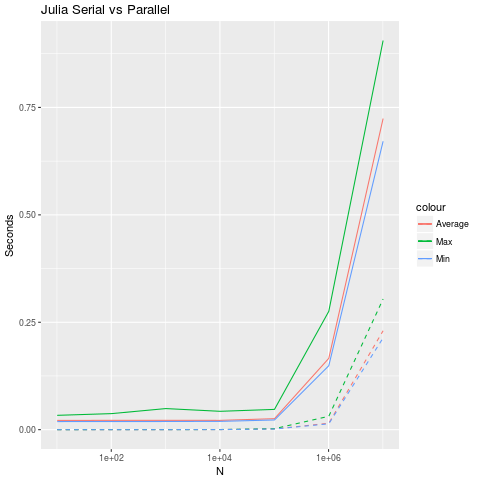
\includegraphics[width=\textwidth]{plot.png}


\begin{table}[ht]
\centering
\caption{Cumulative Sum Performance in OpenMPI C vs. Julia (ms)}
\label{Test-Cases}
\begin{tabular}{|l|c|c|c|c|c|c|}
\hline
Size of Array        & \textbf{\begin{tabular}[c]{@{}c@{}}Julia \\ Average\end{tabular}} & \textbf{\begin{tabular}[c]{@{}c@{}}OpenMPI \\ Average\end{tabular}} & \textbf{\begin{tabular}[c]{@{}c@{}}Julia\\ Worst Case\end{tabular}} & \textbf{\begin{tabular}[c]{@{}c@{}}OpenMPI \\ Worst Case\end{tabular}} & \textbf{\begin{tabular}[c]{@{}c@{}}Julia \\ Best Case\end{tabular}} & \textbf{\begin{tabular}[c]{@{}c@{}}OpenMPI \\ Best Case\end{tabular}}  \\ \hline
\textbf{10} 		& 20.91 & 17.70   & 28.99    & 40.14  & 18.61  & 10.75\\ \hline
\textbf{100} 		& 20.78 & 23.75   & 40.87    & 49.02  & 18.74  & 10.86\\ \hline
\textbf{1000} 		& 20.86 & 21.84   & 31.87    & 53.15  & 18.60  & 11.41\\ \hline
\textbf{10,000} 	& 21.14 & 21.68   & 31.77    & 43.93  & 18.98  & 10.79\\ \hline
\textbf{100,000} 	& 24.23 & 24.19   & 35.14    & 65.61  & 21.84  & 12.46\\ \hline
\textbf{1,000,000} 	& 161.75 & 40.34  & 272.53   & 69.22  & 149.27 & 28.04\\ \hline
\textbf{10,000,000} & 766.60 & 195.85 & 1,083.26 & 231.74 & 696.51 & 170.66\\ \hline

\end{tabular}
\end{table}


	As is apparent Table 3, Julia, when compared to the C version of OpenMPI, does very well at lower sample sizes. The high performance at low sample sizes indicates several things. First of all, Julia's parallelization through message passing is at least on par if not better than that of OpenMPIi in terms of latency. This comes from the fact that we send more messages with Julia because of the requirement of both function calls and variable requests to be done through message passing, yet we still see a performance on par, if not better than the C implementation of MPI in some cases. However, these tests were performed entirely locally with both implementations. As a result latency over messages is extremely low. Because of the greater volume of messages required by Julia, the performance gain would likely diminish when working on a network cluster, especially if it is not particularly low latency. What is particularly interesting is the across the board better performance ceiling of Julia at low sample sizes. This could be due to less overhead of initialization of nodes for parallelization. Where MPI requires initialization and a variety of variables to be set for each node, Julia only invokes the information required per node from the master node and goes from there.

	Interestingly, Julia appears to struggle when given larger tasks compared to MPI. Due to the very sudden spike in time of the algorithm when compared to MPI, we know that for some reason, the large array size is causing a bottleneck. This is most likely one of two things, either the Message Passing interface of Julia does not have very high throughput, or Julia is having issues performing large-scale array comutations. It seems highly unlikely that Julia cannot handle arrays of that large a size given the focus on large array computation by the developers. One issue at hand that could be due to the large array size is vectorization, which causes slowdown in Julia due to extremely efficient for loop implementation.\footnote{Dahua Lin, Sep. 4, 2013,\url{https://julialang.org/blog/2013/09/fast-numeric}} Despite the issue of vectorization though, each of the potentially vectorized commands are in fact specific calls for large arrays. Thus it seems doubtful the Julia developers would write their built in reduction functions without large arrays in mind. Given this information, it seems likely that the implementation of message passing, though low on latency, does not support very high throughput. The reasoning for this is with small sample sizes, the latency of the execution as a whole will be most strongly affected by the latrency and the throughput can be ignored. However, as you grow, if you have a lower throughput system, the bottleneck will begin to grow your overall delay by a wider margin as happened with Julia vs MPI. 


\printbibliography

\listoftodos

\end{document}
